\chapter{Background}
\label{chapter:background} 

The problem must have some background, otherwise it is not
interesting.  You can explain the background here. Probably you should
change the title to something that describes more the content of this
chapter. Background consists of information that help other masters of
the same degree program to understand the rest of the thesis.

Transitions mentioned in Section~\ref{section:structure} are used also
in the chapters and sections. For example, next in this chapter we
tell how to use English language, how to find and refer to sources,
and enlight different ways to include graphics in the thesis\cite{dean2008mapreduce}.

\section{Smart grids }

Energy industry across the globe is facing numerous challenges. There is a huge pressure from regulatory authorities and environmental organizations to reduce carbon foot print, expand their renewable energy portfolios, and take energy conservation measures. The demand response (DR)\footnote{Demand Respose(DR); Changes in electric usage by end-use customers from their normal consumption patterns in response to changes in the price of electricity over time, or to incentive payments designed to induce lower electricity use at times of high wholesale market prices or when system reliability is jeopardized.} and its impacts on consumer behaviour requires rapid adaptations in energy service providers business models. According to United States Federal Energy Regulatory Commission (FERC) , ``Demand response can provide competitive pressure to reduce wholesale power prices; increases awareness of energy usage; provides for more efficient operation of markets; mitigates market power; enhances reliability; and in combination with certain new technologies, can support the use of renewable energy resources, distributed generation, and advanced metering. Thus, enabling demand-side resources, as well as supply-side resources, improves the economic operation of electric power markets by aligning prices more closely with the value customers place on electric power''\cite{federal2008assessment}.  
Traditionally, power system participants have been strictly producers or consumers of electricity. The demand response and reliability issue with conventional electric power distribution models on consumer side are causing a major trend in motivating consumers to produce electricity at domestic level mostly using the renewable energy production methods.  `` Prosumer'' is an emerging term used for an economically motivated entity that: \cite{grijalva2011prosumer}
\begin{itemize}
\item Consumes, produces, and stores power,
\item Operates or owns a power grid small or large, and hence transports electricity, and
\item Optimizes the economic decisions regarding its
\end{itemize}

The current energy grids support unidirectional distribution models and are centralized in nature.  They are very limited to handle the prosumer needs. Line loses and hierarchical topology makes them less reliable. They usually become bottle neck when rapid adaptations are required for demand response. Farhangi, 2010 define smarts grids as ``The next-generation electricity grid, expected to address the major shortcomings of the existing grid. In essence, the smart grid needs to provide the utility companies with full visibility and pervasive control over their assets and services. The smart grid is required to be self-healing and resilient to system anomalies. And last but not least, the smart grid needs to empower its stakeholders to define and realize new ways of engaging with each other and performing energy transactions across the system'' \cite{farhangi2010path}.

In our research, we used data collected from smart metering devices as part of a pilot smart grid project. The data was used to generate analysis that recommends improvement for both demand and supply side to achieve energy efficiency as well as provide understanding to enable correct decision to adapt for demand response.


\section{CIVIS Poject}

CIVIS is the abbreviated name for ``Cities as drivers of social change'' project under European Union 7th framework. It is a part of the programme for optimising energy systems in smart cities. CIVIS project is a collaborative effort of 10 European universities) \footnote{1. Associazione Trento RISE, Italy 2. Aalto university, Finland 3. Imperial College London, UK 4. ENEL Foundation, Italy 5. Instituto Superior Técnico, Portugal 6.Karlsruhe Institute of Technology, Germany 7.Kungliga Tekniska Hogskolan, Sweden 8.SANTER REPLY SpA Italy 9.Nederlandse Organisatie voor toegepast Natuurwetenschappelijkonderzoek, Netherlands 10. Delft University of Technology,Netherlands  }. It aims to embed the social aspect into the advancements of energy technology. To unleash the full potential of this vision, smart grids need to be coupled with broader social and cultural considerations and understood as complex socio-techno-economic systems with multiple decision making layers that are in effect at the physical, cyber, social, and policy \cite{civisproposal}.

ICT acts as one of the main enabler of smart grids,  distributed  and bidirectional information flow models.  On the other hand ICT also provides a lot of new mediums for social aggregation e.g. internet based social media. CIVIS projects tends to connect these two different dimensions with innovative ICT solutions. An integrated approach to energy efficiency is the basic manifesto of CIVIS project. \cite{civisproposal}

Understanding energy usage patterns and benchmarking energy efficiency performance of small units within cities are some preliminary items in list of CIVIS objectives. Within scope of our research we analyze energy data to understand the consumption patterns and try to evaluate various factors that can effect directly or indirectly on the usage patterns. We also try to classify the building on basis of energy efficiency and try to test the sensitivity of energy efficiency with respect to factors that can cause shift in usage patterns. For the CIVIS project aim of social aspect integration, we also present an ICT application framework that can be used to collect and analyse social media data. However the analysis of that data is not within the scope of this research. 


\section{Green Campus Initiative}

Green campus initiative is a project by VTT  ``Technical Research Centre of Finland'' . It is part of EcoCampus 2030 program. EcoCampus is an attempt to contribute to increased energy efficiency in districts and buildings by innovative management and control systems capable to optimize the local consumption without compromising the indoor environment, occupant comfort and building performance, and by introducing new ICT enabled business models \cite{ greencampus}. The vision of the program is to realize a net zero energy model for a world class research, development and educational facility. Program focuses on co-designing this model with user by educating them and then collecting feedbacks for improvement. The main aim is to gain energy efficiency by building infrastructure in the building units that can make them self sustain for future requirements. The aim is build to build a performance based ecosystem that can help both consumers and producers to adapt with demand response.

Green campus initiative is a pilot project for EcoCampus program  in which VTT has installed smart devices inside Aalto University, Finland campus building in cities of Espoo and Helsinki. These specialized devices contained smart metering for energy consumption and indoor environment monitoring sensors.  The data used for analysis in our research was collected from 100 buildings as test sites. The data includes hourly consumption of electricity and electricity used for heating. For one of the test sites VTT provided us the data with the details up to use of  respective electric devices used in that site. This was achieved using smart NIALM \footnote{ NIALM stands for non-intrusive appliance load monitoring,  is a process for analysing changes in the voltage and current going into a house and deducing what appliances are used in the house as well as their individual energy consumption }\cite{ hart1992nonintrusive} meters that can distinguish between different electric devices used on basis of their signal thumb print.

Apart from providing the data, VTT green campus researchers have also helped us in formulating the use cases for this thesis research.


\section{Big Data Analytics}

Big data analytics is application of advance data analytics techniques on large volumes of data. Advance analytics is a generalized term used for data analysis techniques like statistical analysis, data mining, machine learning, natural language processing, text mining and data visualization etc \cite{russom2011big}. Although volume of the data is a widely used factor for qualification of a data set as big data but when it come to big data analytics there few other important attributes i.e. variety, velocity, valuation and veracity. The concept of 3Vs (volume, variety and velocity) of data was first given by an analyst, Doug Laney from Gartner  in a 2001 MetaGroup research publication, ``3D data management: Controlling data volume, variety and velocity''\cite{laney20013d}.  Gartner used this concept to formulate a data magnitude index that can support decision making for selection of the solutions for tackling big data challenge on use case base. This concept is shown in Figure~\ref{fig:3Vs} below

\begin{figure}[ht]
  \begin{center}
    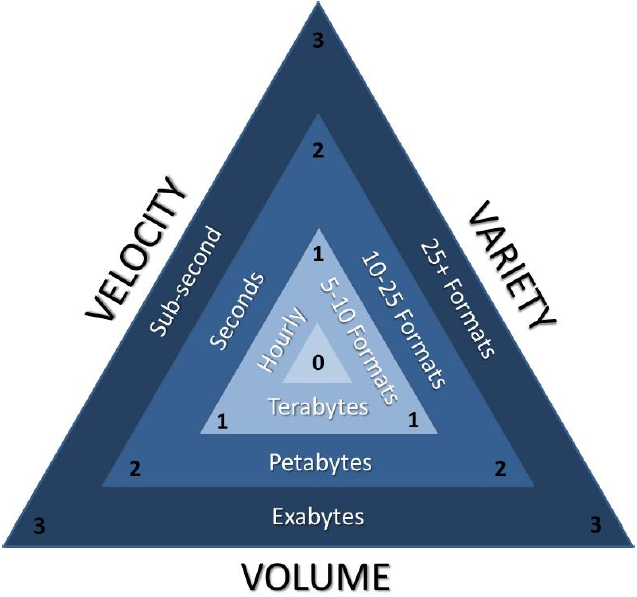
\includegraphics[width=0.7\textwidth]{images/3Vs.png}
    \caption{Gartner 3Vs of data and data magnitude index.}
    \label{fig:3Vs}
  \end{center}
\end{figure}

Number 0 to 3 represents the scale of data that you perceive on each dimension. Adding them together for a big data case can provide the data magnitude index. This method provides some basis for quantifying the data for big data qualification, However it is not providing a definitive model as it allows presumptions to scale the data. Valuation and veracity are two other factors that are being used widely along with Gartner's 3V. Valuation supports the decision making by considering the value of outcomes against the efforts required to collect, manage, process and analyse huge amounts of data.  While veracity refers to ambiguity in the data that can cause complexity. There is no standard definition of big data but most of the attempts to define big data can be associated with these five factors that we have discussed.

As a matter of fact, we are not attempting to provide a definition of big data as part of this thesis or stating any criteria for qualification of a data set as big data. Instead we shall be proposing an advance analytics model that should be capable enough to handle big data as well other smaller data sets on need basis. The modular architecture of the model platform can be tweaked to handle volume, variety, velocity, and veracity on need basis while trying to maximize the valuation for the use case. 

